\documentclass{article}

\usepackage[T1]{fontenc}
\usepackage{graphicx}
\usepackage{color}
\usepackage[parfill]{parskip}
\usepackage{titlesec}
\usepackage{titling}
\usepackage{anyfontsize}

\titleformat*{\subsection}{\fontsize{11}{14}\bfseries}

\setlength{\droptitle}{-2em}

\newcommand{\todo}[1]{\textcolor{red}{[#1]}}

\newcommand{\definepoints}[2]{%
  \expandafter\newcommand\csname rmk-#1\endcsname{#2}%
}
\newcommand{\points}[1]{\csname rmk-#1\endcsname}

\definepoints{q1}{8}
\definepoints{q2}{6}


\definepoints{q3}{6}
\definepoints{q3partial1}{3}
\definepoints{q3partialGrad1}{3}
\definepoints{q3partialGrad2}{5}

\definepoints{q4}{6}
\definepoints{q4partialGrad1}{3}
\definepoints{q4partialGrad2}{5}


\title{AI Challenge 4: Adversarial Search}
\date{}
\author{COSC4550/COSC5550\\
Artificial Intelligence\\
University of Wyoming}

\begin{document}

\maketitle




\section{Overview}
In this project, you will design agents for the classic version of Pac-Man, including ghosts. Along the way, you will implement minimax with alpha-beta pruning and try your hand at evaluation function design.

\begin{figure}[h]
\centering
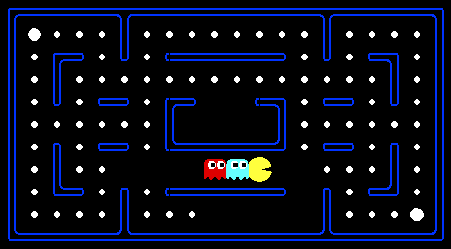
\includegraphics[width=0.8\textwidth]{pacman_multi_agent.png}
\caption{The full Pacman game.}
\label{fig:screen}
\end{figure}

\noindent
\textit{Acknowledgment: This assignment is based on the one created by Dan Klein and John DeNero given as part of Berkeley's CS188 course. This assignment was also inspired by the modifications made by Peter Stone in his CS343 course of 2012. 
We thank Dan and John for creating the assignment and granting the permission to use it and we thank Peter for the ideas on how to adapt the assignment for this course.}


\newpage
\subsection{Chapters}
Chapters are from the book `Artificial Intelligence, A Modern Approach', third edition, by Stuart Russel and Peter Norvig. The relevant chapter for this challenge is chapter 5, sections 1, 2, and 3. The most relevant sub-sections are 5.2.1 (The minimax algorithm) and 5.3 (Alpha-Beta Pruning).


\subsection{Program files}
The archive for this challenge contains a number of Python files. These files have been tested on, and should work with, Python version 2.7.3 and Python version 2.6.6. More recent versions of Python 2.x probably work as well, but these files do not work with Python 3.x.

Once again, the code has not changed much from the previous project, but please start with a fresh installation, rather than intermingling files from challenge 3. You can, however, use your \emph{search.py} in any way you want. The important files for this challenge are:

\vspace{10pt}
\noindent
\begin{tabular}{r p{0.70\textwidth}}
\emph{multiAgents.py} & This file should be extended with your implementations of the adversarial Pacman agents. \\
\emph{pacman.py} & The main file that runs Pacman games. This file describes a Pacman GameState type, which you will use in this project.\\
\emph{game.py} & The logic behind how the Pacman world works. This file describes several supporting types like AgentState, Agent, Direction, and Grid.\\
\emph{util.py} & Useful data structures for implementing search algorithms.\\
\emph{autograder.py} & You do not need to examine this file, but it can help you test your \emph{minimax} and \emph{alpha-beta} algorithms.
\end{tabular}
\vspace{10pt}

You can test whether everything is working by playing a game of classic Pacman using:

\begin{verbatim}
python pacman.py
\end{verbatim}

\subsubsection{The autograder}
For question 1 and 2 of this challenge we also provide you with an autograder, which will check the correctness of your algorithm in various scenarios. Note that the autograder is not perfect and you might still have some bugs in your code even if you pass all tests. It is also possible, that the autograder will `fail' a correct solution because of a minor implementation difference. If you feel that the autograder is mistakenly failing a correct solution, please let us know, and we will try to update the autograder to account for your case. That said, the autograder has been tested by many students before you, so it is quite likely that the autograder is working as intended, and that you will have to debug your solution.

The autograder has various options which might help you to debug your program. Useful options include \texttt{-p} which will print the test case before doing the test and \texttt{-{}-no-graphics} which will not display the Pacman game for faster grading. To see all options us \texttt{-h}.

Note that the games the autograder shows are controlled by the autograder, not by your agent, meaning that the autograder games will always be the same, regardless of the actions you agent chooses. This is done so we can compare the actions of your agent with the actions known to be optimal. To see your own agent in action, run the game directly with the \emph{pacman.py} commands.

\subsection{Deliverables}
For this challenge you should submit your version of \emph{multiAgents.py}. Please rename your file to \emph{[yourname]\_multiAgents.py} before handing it in. You are also allowed to send any number of supporting files (like \emph{search.py}, etc.) but please do not change or send any of our original files.

\textbf{Important:} Make absolutely sure that your implementation will run all questions without any modifications being necessary on our part. It should run on either python 2.7.3 or python 2.6.6 and, when in doubt, you can always test your implementation on hive. You will only receive partial credit for implementations that do not run.

To run your solution on hive, first copy your project to hive (hive.cs.uwyo.edu) using any protocol accepted by hive (such as scp), then ssh onto hive and run your solution. Do not forget to use the \texttt{-q} (for \emph{pacman.py}) or \texttt{-{}-no-graphics} (for \emph{autograder.py}) option, as you will not have a display on hive and the program will crash without them.

\section{Questions}

\subsection{Question 1 (\points{q1} points)} 
You will write an adversarial search agent in the provided \emph{MinimaxAgent} class stub in \emph{multiAgents.py}. Your minimax agent should work with any number of ghosts, so you'll have to write an algorithm that is slightly more general than what appears in the textbook. In particular, your minimax tree will have multiple min layers (one for each ghost) for every max layer. Note that the way the game progresses is, in a round robin fashion, where Pacman takes a step, then ghost1 takes a step, then ghost2 takes a step, ..., then Pacman takes a step, and so on.

Your code should also expand the game tree to an arbitrary depth. Score the leaves of your minimax tree with the supplied \emph{self.evaluationFunction}, which defaults to \emph{scoreEvaluationFunction}. \emph{MinimaxAgent} extends \emph{MultiAgentSearchAgent}, which gives access to \emph{self.depth} and \emph{self.evaluationFunction}. Make sure your minimax code makes reference to these two variables where appropriate as these variables are populated in response to command line options. Test your code on the \emph{minimaxClassic} maze for up to four plies deep. 

\begin{verbatim}
python pacman.py -p MinimaxAgent -l minimaxClassic -a depth=1
python pacman.py -p MinimaxAgent -l minimaxClassic -a depth=2
python pacman.py -p MinimaxAgent -l minimaxClassic -a depth=3
python pacman.py -p MinimaxAgent -l minimaxClassic -a depth=4
\end{verbatim}

You can use the autograder on question 1 with the following command:

\begin{verbatim}
python autograder.py -q q1
\end{verbatim}


\textbf{Important:} A single search ply is considered to be one Pacman move and all the ghosts' responses, so depth 2 search will involve Pac-Man and each ghost moving two times.


\subsubsection{Hints and Observations}

\begin{itemize}

\item The minimax values of the initial state in the \emph{minimaxClassic} layout are 9, 8, 7, -492 for depths 1, 2, 3 and 4 respectively, according to the default \texttt{scoreEvaluationFunction} (that is, these are the final scores Pac-Man expects to receive if the opponents play optimally). Note that, because the opponents do not play optimally, your minimax agent will often win (600/1000 games for us) despite the dire prediction of depth 4 minimax.

\item To increase the search depth achievable by your agent, remove the Directions.STOP action from Pacman's list of possible actions. Depth 2 should be pretty quick, but depth 3 or 4 will be slow. Don't worry, the next question will speed up the search somewhat.

\item Pacman is always agent 0, and the agents move in order of increasing agent index.
All states in minimax should be \emph{GameStates}, either passed in to \emph{getAction} or generated via \emph{GameState.generateSuccessor}.

\item On larger boards such as \emph{openClassic} and \emph{mediumClassic} (the default), you'll find Pacman to be good at not dying, but quite bad at winning. He'll often thrash around without making progress. He might even thrash around right next to a dot without eating it because he doesn't know where he'd go after eating that dot. Don't worry if you see this behavior, question 3 will clean up most of these issues.

\item When Pacman believes that his death is unavoidable, he will try to end the game as soon as possible because of the constant penalty for living. Sometimes, this is the wrong thing to do with random ghosts, but minimax agents always assume the worst. 

%Once you have implemented minimax you can try it on the following maze: 

%\begin{small}
%\begin{verbatim}
%python pacman.py -p MinimaxAgent -l trappedClassic -a depth=3
%\end{verbatim}
%\end{small}
%
%Make sure you understand why Pac-Man rushes the closest ghost in this case.

\item The game score, which is the evaluation function for this challenge, works by adding and subtracting from the current game score (which starts at zero) in the following way: 
\begin{itemize}
\item[] $-1$ for each time-step
\item[]  $+10$ for each food item eaten
\item[]  $+200$ for eating ghosts
\item[]  $+500$ for winning
\item[]  $-500$ for losing
\end{itemize}



\end{itemize}

\subsubsection{Grading: \points{q1} points}
You will get full credit if you correctly implement minimax search (use the autograder to test that it does!). This means that, for every possible state, your agent should return one of the actions that provides the highest score according to the minimax algorithm using the default \emph{scoreEvaluationFunction}. In case of ties your agent may chose any of the best actions.


\subsection{Question 2 (\points{q2} points)}
Make a new agent that uses alpha-beta pruning to more efficiently explore the minimax tree, in AlphaBetaAgent. Again, your algorithm will be slightly more general than the pseudo-code in the textbook, so part of the challenge is to extend the alpha-beta pruning logic appropriately to multiple minimizer agents.

You should see a speed-up (perhaps depth 3 alpha-beta will run as fast as depth 2 minimax). Ideally, depth 3 on smallClassic should run in just a few seconds per move or faster.

\begin{verbatim}
python pacman.py -p AlphaBetaAgent -a depth=3 -l smallClassic
\end{verbatim}

The \emph{AlphaBetaAgent} minimax values should be identical to the \emph{MinimaxAgent} minimax values, although the actions it selects can vary because of different tie-breaking behavior. Again, the minimax values of the initial state in the \emph{minimaxClassic} layout are 9, 8, 7 and -492 for depths 1, 2, 3 and 4 respectively. As for the previous question you can use the autograder to check the correctness of your algorithm:

\begin{verbatim}
python autograder.py -q q2
\end{verbatim}

\subsubsection{Grading: \points{q2} points}
You will get full credit if you correctly implement minimax search with alpha-beta pruning. This means that, in addition to always returning a `best' action, your algorithm should explore a minimum number of states according to the alpha-beta pruning algorithm. Note that, for the purpose of automatic grading, the states explored are determined by calls to \emph{gameState.generateSuccessor}, so you have to make sure that you call this function for exploring states and that you only call it for states that you actually explore. Use the autograder to check that you don't expand unnecessary states.



\subsection{Question 3 (\points{q3} points)} 
Write a better evaluation function for pacman in the provided function \emph{betterEvaluationFunction}. You may use any tools at your disposal for evaluation, including your search code from the last project. With depth 2 search, your evaluation function should clear the \emph{smallClassic} layout with two random ghosts more than half the time and still run at a reasonable rate.

Because of the variance in the performance on this task we will test your code on a batch of 50 runs with an initial seed of 1 using the \texttt{-s 1} option. Note that this does \emph{not} fix the seed for each run as your second run will take the state of the random number generator left by your first run and use it to produce numbers for the second run. This means that each of the 50 runs will be different and, more importantly, that if one run goes differently because of a change you made, all subsequent runs might be different as well. The command we'll use is listed below.

\begin{footnotesize}
\begin{verbatim}
python pacman.py -l smallClassic -p AlphaBetaAgent -a evalFn=better -s 1 -q -n 50
\end{verbatim}
\end{footnotesize}


\subsubsection{Hints and Observations}

\begin{itemize}
\item To see which information you have available by default check the \emph{GameState} class in \emph{pacman.py}.

\item As noted in question 1, our opponents do not play optimally. While this might seem like a fundamental problem for minimax search, you can use the evaluation function to circumvent this problem by giving higher values to states in which Pac-Man has at least has some chance of survival, or to states in which Pac-Man survived longer.

\item When all states that Pac-Man can `see' with the current search depth have similar values he will often refuse to move or thrash around in a very small space. Make sure your evaluation function provides a way to identify states that at least bring Pac-Man closer to the goal of winning the game, even when there does not seem to be a direct benefit. 

\item One way you might want to write your evaluation function is to use a linear combination of features. That is, compute values for features about the state that you think are important, and then combine those features by multiplying them by different values and adding the results together. You might decide what to multiply each feature by based on how important you think it is.

\item Winning a game will usually give you a score of about 950. To get a higher score your agent also has to capture some ghosts before finishing the game.
\end{itemize}

\subsubsection{Grading: \points{q3} points}
To get any credit Pacman should be winning more than half the time with search depth 2 on the \emph{smallClassic} layout with 2 random ghosts and a set of 50 games may not take more than 30 minutes without graphics (if you are unsure whether your algorithm will run in the allotted time you can check this yourself by running it on hive). If you meet these requirements you'll get points depending on your average score.


\vspace{10pt}
\noindent
\begin{tabular}{lll}
\textbf{Average score}                & \textbf{Points COSC 4550} & \textbf{Points COSC 5550}\\
$score < 900$                         & \points{q3partial1}        & \points{q3partialGrad1}\\
$900 \leq score < 1100$               & \points{q3}               & \points{q3partialGrad2}\\
$1100 \leq score < 1300$              & +0.5 extra credit         & \points{q3}\\
$1300 \leq score < 1586$              & +0.5 extra credit         & +1 extra credit\\
$1586 \leq score$ (current record)    & +1 extra credit           & +1 extra credit\\
\end{tabular}
\vspace{10pt}



\subsection{Question 4 (\points{q4} points, COSC5550 mandatory, COSC4550 bonus): Ultimate Pacman} 
\noindent \emph{(Mandatory for those enrolled in the graduate student version of the class. Bonus points for undergraduates)}

Now it is time for Pacman to show off how good he has become. Pacman will face off against more intelligent opponents in a trickier maze. In particular, the ghosts will actively chase Pacman instead of wandering around randomly, and the maze features more twists and dead-ends, but also extra pellets to give Pacman a fighting chance. You're free to have Pacman use any search procedure, search depth, and evaluation function you like. The only limit is that the set of 10 games can last a maximum of 30 minutes in total (with graphics off, you can check your code on hive), so be sure to use your computation wisely. Because of the high variance in this maze we will run your code with the fixed seed of 1 for a set of runs. To be more precise we'll run your program with the following command:

\begin{scriptsize}
\begin{verbatim}
python pacman.py -l ultimateClassic -p UltimateAgent -g DirectionalGhost -s 1 -q -n 10
\end{verbatim}
\end{scriptsize}

\subsubsection{Hints and Observations}

\begin{itemize}
\item The seed is not reset before each game, meaning your agent will have to perform well on ten different games!
\item Note that you will have to set your evaluation function and depth in your code as they will not be provided by command line arguments.
\item The success of Pacman for this question is determined by score and score alone. Pacman does not have to win any games as long as his score is good enough.
\end{itemize}


\subsubsection{Grading: \points{q4} points}
To get full credit the full set of 10 games my not last any longer than 30 minutes. If you meet these requirements you will get credit based upon your average score.

\vspace{10pt}
\noindent
\begin{tabular}{lll}
\textbf{Average score}              & \textbf{Points COSC 4550}     & \textbf{Points COSC 5550}\\
$score < 1100$                      &                               & \points{q4partialGrad1}\\
$1000 \leq score < 1200$            & +0.5 extra credit             & \points{q4partialGrad2}\\
$1200 \leq score < 1700$            & +0.5 extra credit             & \points{q4}\\
$1700 \leq score < 2488$            & +0.5 extra credit             & +1 extra credit\\
$2488 \leq score$ (current record)  & +0.5 extra credit             & +1 extra credit\\
\end{tabular}
\vspace{10pt}

\section{FAQ}

\begin{itemize}
\item[Q:] \emph{What does it mean when a ghost has no legal actions?}
\item[A:] It means that the game has ended.
\item[]

\item[Q:] \emph{I am getting the following error when running the autograder: "AttributeError: `MultiagentTreeState' object has no attribute `getPacmanPosition'", what is wrong?}
\item[A:] The problem is that you call the method \texttt{getPacmanPosition} on a game-state, but not all autograder game-states have a Pacman position (the \texttt{MultiagentTreeState} is a search tree for example). As such, avoid calling \texttt{getPacmanPosition}, and use the proper functions like \texttt{getLegalActions} and \texttt{generateSuccessor} instead.
\item[]



\item[Q:] \emph{I am getting the following error when running the autograder: "getScore() called on non-terminal state or before maximum depth achieved", what is wrong?}
\item[A:] While you can evaluate every state in the Pacman game, you can only evaluate leaf nodes or nodes at the maximum depth in the autograder. As such, make sure you do not call the \texttt{getScore} method on anything that isn't at maximum depth and that isn't a leaf node.
\item[]

\item[Q:] \emph{How do I create a good evaluation function?}
\item[A:] While there are many things that go into a good evaluation function, there are three things your evaluation function should always do:
\begin{itemize}
\item Always provide direction: if no dots are near, make sure you give some score for moving towards them.
\item Smooth gradients towards the end of the game: sitting next to a dot should never give you more score than collecting it. 
\item Incentive to finish the game: there should be some penalty for waiting around.
\end{itemize}

Also, remember that your minimax algorithm will look ahead. As such, do not give a high score for collecting the dot, but instead give a high score for any game in which the dot is no longer there.
\item[]
\end{itemize}

\end{document}
